% Options for packages loaded elsewhere
\PassOptionsToPackage{unicode}{hyperref}
\PassOptionsToPackage{hyphens}{url}
\PassOptionsToPackage{dvipsnames,svgnames,x11names}{xcolor}
%
\documentclass[
  12pt,
  letterpaper,
  DIV=11,
  numbers=noendperiod]{scrartcl}

\usepackage{amsmath,amssymb}
\usepackage{iftex}
\ifPDFTeX
  \usepackage[T1]{fontenc}
  \usepackage[utf8]{inputenc}
  \usepackage{textcomp} % provide euro and other symbols
\else % if luatex or xetex
  \usepackage{unicode-math}
  \defaultfontfeatures{Scale=MatchLowercase}
  \defaultfontfeatures[\rmfamily]{Ligatures=TeX,Scale=1}
\fi
\usepackage{lmodern}
\ifPDFTeX\else  
    % xetex/luatex font selection
    \setmainfont[]{Times New Roman}
\fi
% Use upquote if available, for straight quotes in verbatim environments
\IfFileExists{upquote.sty}{\usepackage{upquote}}{}
\IfFileExists{microtype.sty}{% use microtype if available
  \usepackage[]{microtype}
  \UseMicrotypeSet[protrusion]{basicmath} % disable protrusion for tt fonts
}{}
\makeatletter
\@ifundefined{KOMAClassName}{% if non-KOMA class
  \IfFileExists{parskip.sty}{%
    \usepackage{parskip}
  }{% else
    \setlength{\parindent}{0pt}
    \setlength{\parskip}{6pt plus 2pt minus 1pt}}
}{% if KOMA class
  \KOMAoptions{parskip=half}}
\makeatother
\usepackage{xcolor}
\setlength{\emergencystretch}{3em} % prevent overfull lines
\setcounter{secnumdepth}{5}
% Make \paragraph and \subparagraph free-standing
\makeatletter
\ifx\paragraph\undefined\else
  \let\oldparagraph\paragraph
  \renewcommand{\paragraph}{
    \@ifstar
      \xxxParagraphStar
      \xxxParagraphNoStar
  }
  \newcommand{\xxxParagraphStar}[1]{\oldparagraph*{#1}\mbox{}}
  \newcommand{\xxxParagraphNoStar}[1]{\oldparagraph{#1}\mbox{}}
\fi
\ifx\subparagraph\undefined\else
  \let\oldsubparagraph\subparagraph
  \renewcommand{\subparagraph}{
    \@ifstar
      \xxxSubParagraphStar
      \xxxSubParagraphNoStar
  }
  \newcommand{\xxxSubParagraphStar}[1]{\oldsubparagraph*{#1}\mbox{}}
  \newcommand{\xxxSubParagraphNoStar}[1]{\oldsubparagraph{#1}\mbox{}}
\fi
\makeatother


\providecommand{\tightlist}{%
  \setlength{\itemsep}{0pt}\setlength{\parskip}{0pt}}\usepackage{longtable,booktabs,array}
\usepackage{calc} % for calculating minipage widths
% Correct order of tables after \paragraph or \subparagraph
\usepackage{etoolbox}
\makeatletter
\patchcmd\longtable{\par}{\if@noskipsec\mbox{}\fi\par}{}{}
\makeatother
% Allow footnotes in longtable head/foot
\IfFileExists{footnotehyper.sty}{\usepackage{footnotehyper}}{\usepackage{footnote}}
\makesavenoteenv{longtable}
\usepackage{graphicx}
\makeatletter
\newsavebox\pandoc@box
\newcommand*\pandocbounded[1]{% scales image to fit in text height/width
  \sbox\pandoc@box{#1}%
  \Gscale@div\@tempa{\textheight}{\dimexpr\ht\pandoc@box+\dp\pandoc@box\relax}%
  \Gscale@div\@tempb{\linewidth}{\wd\pandoc@box}%
  \ifdim\@tempb\p@<\@tempa\p@\let\@tempa\@tempb\fi% select the smaller of both
  \ifdim\@tempa\p@<\p@\scalebox{\@tempa}{\usebox\pandoc@box}%
  \else\usebox{\pandoc@box}%
  \fi%
}
% Set default figure placement to htbp
\def\fps@figure{htbp}
\makeatother
% definitions for citeproc citations
\NewDocumentCommand\citeproctext{}{}
\NewDocumentCommand\citeproc{mm}{%
  \begingroup\def\citeproctext{#2}\cite{#1}\endgroup}
\makeatletter
 % allow citations to break across lines
 \let\@cite@ofmt\@firstofone
 % avoid brackets around text for \cite:
 \def\@biblabel#1{}
 \def\@cite#1#2{{#1\if@tempswa , #2\fi}}
\makeatother
\newlength{\cslhangindent}
\setlength{\cslhangindent}{1.5em}
\newlength{\csllabelwidth}
\setlength{\csllabelwidth}{3em}
\newenvironment{CSLReferences}[2] % #1 hanging-indent, #2 entry-spacing
 {\begin{list}{}{%
  \setlength{\itemindent}{0pt}
  \setlength{\leftmargin}{0pt}
  \setlength{\parsep}{0pt}
  % turn on hanging indent if param 1 is 1
  \ifodd #1
   \setlength{\leftmargin}{\cslhangindent}
   \setlength{\itemindent}{-1\cslhangindent}
  \fi
  % set entry spacing
  \setlength{\itemsep}{#2\baselineskip}}}
 {\end{list}}
\usepackage{calc}
\newcommand{\CSLBlock}[1]{\hfill\break\parbox[t]{\linewidth}{\strut\ignorespaces#1\strut}}
\newcommand{\CSLLeftMargin}[1]{\parbox[t]{\csllabelwidth}{\strut#1\strut}}
\newcommand{\CSLRightInline}[1]{\parbox[t]{\linewidth - \csllabelwidth}{\strut#1\strut}}
\newcommand{\CSLIndent}[1]{\hspace{\cslhangindent}#1}

\usepackage{tcolorbox}
\usepackage{amssymb}
\usepackage{yfonts}
\usepackage{bm}


\newtcolorbox{greybox}{
  colback=white,
  colframe=blue,
  coltext=black,
  boxsep=5pt,
  arc=4pt}
  
\newcommand{\sectionbreak}{\clearpage}

 
\newcommand{\ds}[4]{\sum_{{#1}=1}^{#3}\sum_{{#2}=1}^{#4}}
\newcommand{\us}[3]{\mathop{\sum\sum}_{1\leq{#2}<{#1}\leq{#3}}}

\newcommand{\ol}[1]{\overline{#1}}
\newcommand{\ul}[1]{\underline{#1}}

\newcommand{\amin}[1]{\mathop{\text{argmin}}_{#1}}
\newcommand{\amax}[1]{\mathop{\text{argmax}}_{#1}}

\newcommand{\ci}{\perp\!\!\!\perp}

\newcommand{\mc}[1]{\mathcal{#1}}
\newcommand{\mb}[1]{\mathbb{#1}}
\newcommand{\mf}[1]{\mathfrak{#1}}

\newcommand{\eps}{\epsilon}
\newcommand{\lbd}{\lambda}
\newcommand{\alp}{\alpha}
\newcommand{\df}{=:}
\newcommand{\am}[1]{\mathop{\text{argmin}}_{#1}}
\newcommand{\ls}[2]{\mathop{\sum\sum}_{#1}^{#2}}
\newcommand{\ijs}{\mathop{\sum\sum}_{1\leq i<j\leq n}}
\newcommand{\jis}{\mathop{\sum\sum}_{1\leq j<i\leq n}}
\newcommand{\sij}{\sum_{i=1}^n\sum_{j=1}^n}
	
\KOMAoption{captions}{tableheading}
\makeatletter
\@ifpackageloaded{caption}{}{\usepackage{caption}}
\AtBeginDocument{%
\ifdefined\contentsname
  \renewcommand*\contentsname{Table of contents}
\else
  \newcommand\contentsname{Table of contents}
\fi
\ifdefined\listfigurename
  \renewcommand*\listfigurename{List of Figures}
\else
  \newcommand\listfigurename{List of Figures}
\fi
\ifdefined\listtablename
  \renewcommand*\listtablename{List of Tables}
\else
  \newcommand\listtablename{List of Tables}
\fi
\ifdefined\figurename
  \renewcommand*\figurename{Figure}
\else
  \newcommand\figurename{Figure}
\fi
\ifdefined\tablename
  \renewcommand*\tablename{Table}
\else
  \newcommand\tablename{Table}
\fi
}
\@ifpackageloaded{float}{}{\usepackage{float}}
\floatstyle{ruled}
\@ifundefined{c@chapter}{\newfloat{codelisting}{h}{lop}}{\newfloat{codelisting}{h}{lop}[chapter]}
\floatname{codelisting}{Listing}
\newcommand*\listoflistings{\listof{codelisting}{List of Listings}}
\makeatother
\makeatletter
\makeatother
\makeatletter
\@ifpackageloaded{caption}{}{\usepackage{caption}}
\@ifpackageloaded{subcaption}{}{\usepackage{subcaption}}
\makeatother

\usepackage{bookmark}

\IfFileExists{xurl.sty}{\usepackage{xurl}}{} % add URL line breaks if available
\urlstyle{same} % disable monospaced font for URLs
\hypersetup{
  pdfauthor={Jan de Leeuw},
  colorlinks=true,
  linkcolor={blue},
  filecolor={Maroon},
  citecolor={Blue},
  urlcolor={Blue},
  pdfcreator={LaTeX via pandoc}}


\title{Smacof at 50: A Manual\\
Part 1: Introduction}
\author{Jan de Leeuw}
\date{December 9, 2024}

\begin{document}
\maketitle

\renewcommand*\contentsname{Table of contents}
{
\hypersetup{linkcolor=}
\setcounter{tocdepth}{3}
\tableofcontents
}

\sectionbreak

\textbf{Note:} This manual is a working manuscript which will be
expanded/updated frequently. All suggestions for improvement are
welcome. All Rmd, tex, html, pdf, R, and C files are in the public
domain and can be copied, modified, and used by anybody in any way they
see fit. Attribution will be appreciated, but is not required. The files
can be found at \url{https://github.com/deleeuw} in the repositories
smacofCode, smacofManual, and smacofExamples.

\sectionbreak

\section*{Conventions, Notations and Reserved
Symbols}\label{conventions-notations-and-reserved-symbols}
\addcontentsline{toc}{section}{Conventions, Notations and Reserved
Symbols}

I number and label \emph{all} displayed equations. Equations are
displayed, instead of inlined, if and only if one of the following is
true.

\begin{itemize}
\tightlist
\item
  They are important.
\item
  They are referred to elsewhere in the text.
\item
  Not displaying them messes up the line spacing.
\end{itemize}

All code chunks in the text are named. Theorems, lemmas, chapters,
sections, subsections, and so on are also named and numbered. I use the
serial comma.

The dilemma of whether to use ``we'' or ``I'' throughout the book is
solved in the usual way. If I feel that a result is the work of a group
(me, my co-workers, and the giants on whose shoulders we stand) then I
use ``we''. If it's an individual decision, or something personal, then
I use ``I''. The default is ``we'', as it always should be in scientific
writing.

Most of the individual chapters also have some of the necessary
mathematical background material, both notation and results, sometimes
with specific elaborations that seem useful for the book. Sometimes this
background material is quite extensive. Examples are splines,
majorization, unweighting, monotone regression, and the basic Zangwill
and Ostrowski fixed point theorems we need for convergence analysis of
our algorithms.

\subsection*{Spaces}\label{spaces}
\addcontentsline{toc}{subsection}{Spaces}

\begin{itemize}
\item
  \(\mathbb{R}^n\) is the space of all real vectors, i.e.~all
  \(n\)-element tuples of real numbers. Typical elements of
  \(\mathbb{R}^n\) are \(x,y,z\). The element of \(x\) in position \(i\)
  is \(x_i\). Defining a vector by its elements is done with
  \(x=\{x_i\}\).
\item
  \(\mathbb{R}^n\) is equipped with the inner product
  \(\langle x,y\rangle=x'y=\sum_{i=1}^nx_iy_i\) and the norm
  \(\smash{\|x\|=\sqrt{x'x}}\).
\item
  The canonical basis for \(\mathbb{R}^n\) is the \(n-\)tuple
  \((e_1,cdots,e_n)\), where \(e_i\) has element \(i\) equal to \(+1\)
  and all other elements equal to zero. Thus \(\|e_i\|=1\) and
  \(\langle e_i,e_j\rangle=\delta^{ij}\), with \(\delta^{ij}\) the
  Kronecker delta (equal to one if \(i=j\) and zero otherwise). Note
  that \(x_i=\langle e_i,x\rangle\).
\item
  \(\mathbb{R}\) is the real line and \(\mathbb{R}_+\) is the half line
  of non-negative numbers. The postive reals are \(\mathbb{R}_{++}\).
\item
  \(\mathbb{R}^{n\times m}\) is the space of all \(n\times m\) real
  matrices. Typical elements of \(\mathbb{R}^{n\times m}\) are
  \(A,B,C\). The element of \(A\) in row \(i\) and column \(j\) is
  \(a_{ij}\). Defining a matrix by its elements is done with
  \(A=\{a_{ij}\}\).
\item
  \(\mathbb{R}^{n\times m}\) is equipped with the inner product
  \(\langle A,B\rangle=\text{tr} A'B=\sum_{i=1}^n\sum_{j=1}^ma_{ij}b_{ij}\)
  and the norm \(\|A\|=\sqrt{\text{tr}\ A'A}\).
\item
  The canonical basis for \(\mathbb{R}^{n\times m}\) is the \(nm-\)tuple
  \((E_{11},cdots,E_{nm})\), where \(E_{ij}\) has element \((i,j)\)
  equal to \(+1\) and all other elements equal to zero. Thus
  \(\|E_{ij}\|=1\) and
  \(\langle E_{ij},E_{kl}\rangle=\delta^{ik}\delta^{jl}\).
\end{itemize}

\(\text{vec}\) and \(\text{vec}^{-1}\)

\subsection*{Matrices}\label{matrices}
\addcontentsline{toc}{subsection}{Matrices}

\begin{itemize}
\item
  \(a_{i\bullet}\) is row \(i\) of matrix \(A\), \(a_{\bullet j}\) is
  column \(j\).
\item
  \(a_{i\star}\) is the sum of row \(i\) of matrix \(A\),
  \(a_{\star j}\) is the sum of column \(j\).
\item
  \(A'\) is the transpose of \(A\), and \(\text{diag}(A)\) is the
  diagonal matrix with the diagonal elements of \(A\). The inverse of a
  square matrix \(A\) is \(A^{-1}\), the Moore-Penrose generalized
  inverse of any matrix \(A\) is \(A^+\). The transpose of the inverse,
  and the inverse of the transpose, are \(A^{-T}\).
\item
  If \(A\) and \(B\) are two \(n\times m\) matrices then their Hadamard
  (or elementwise) product \(C=A\times B\) has elements
  \(c_{ij}=a_{ij}b_{ij}\). The Hadamard quotient is \(C=A/B\), with
  elements \(c_{ij}=a_{ij}/b_{ij}\). The Hadamard power is
  \(A^{(k)}=A^{(p-1)}\times A\).
\item
  DC matrices. Centering matrix. \(J_n=I_n-n^{-1}E_n\). We do not use
  the subscripts if the order is obvious from the context.
\item
  Matrices of matrices. Partitioned matrices. \(A_{ij}\) and thus
  \(\{A_{ij}\}_{kl}\).
\item
  Direct sum and Product
\end{itemize}

\subsection*{Functions}\label{functions}
\addcontentsline{toc}{subsection}{Functions}

\begin{itemize}
\item
  \(f,g,h,\cdots\) are used for functions or mappings.
  \(f:X\rightarrow Y\) says that \(f\) maps \(X\) into \(Y\).
\item
  \(\sigma\) is used for all real-valued least squares loss functions.
\end{itemize}

\subsection*{MDS}\label{mds}
\addcontentsline{toc}{subsection}{MDS}

\begin{itemize}
\item
  \(\Delta=\{\delta_{ij\cdots}\}\) is a matrix or array of
  dissimilarities.
\item
  \(\langle \mathbb{X},d\rangle\) is a metric space, with
  \(d:\mathcal{X}\otimes\mathcal{X}\rightarrow\mathbb{R}_+\) the
  distance function. If \(X\) is is an ordered n-tuple
  \((x_1,\cdots,x_n)\) of elements of \(\mathcal{X}\) then \(D(X)\) is
  \(\{d(x_i,x_j)\}\), the elements of which we also write as
  \(d_{ij}(X)\).
\item
  Summation over the elements of vector \(x\in\mathbb{R}^n\) is
  \(\sum_{i=1}^n x_i\). Summation over the elements of matrix
  \(A\in\mathbb{R}^{n\times m}\) is \(\sum_{i=1}^n\sum_{j=1}^m a_{ij}\).
  Summation over the elements above the diagonal of \(A\) is
  \(\mathop{\sum\sum}_{1\leq i<j\leq n}a_{ij}\).
\item
  Conditional summation is, for example,
  \(\sum_{i=1}^n \{x_i\mid x_i>0\}\).
\end{itemize}

\sectionbreak

\section*{Preface}\label{preface}
\addcontentsline{toc}{section}{Preface}

This manual is definitely \emph{not} an impartial and balanced review of
all of multidimensional scaling (MDS) theory and history. It emphasizes
computation, and the mathematics needed for computation. In addition, it
is a summary of over 50 years of MDS work by me, either solo or together
with my many excellent current or former co-workers and co-authors. It
is heavily biased in favor of the smacof formulation of MDS (De Leeuw
(\citeproc{ref-deleeuw_C_77}{1977}), De Leeuw and Heiser
(\citeproc{ref-deleeuw_heiser_C_77}{1977}), De Leeuw and Mair
(\citeproc{ref-deleeuw_mair_A_09c}{2009}), Mair, Groenen, and De Leeuw
(\citeproc{ref-mair_groenen_deleeuw_A_22}{2022})), and the corresponding
majorization (or MM) algorithms. And, moreover, I am shamelessly
squeezing in as many references to my published and unpublished work as
possible, with links to the corresponding pdf's if they are available.
Thus this book is also a jumpstation into my bibliography.

I have not organized the book along historical lines because most of the
early techniques and results have been either drastically improved or
completely abandoned. Nevertheless, some personal historical perspective
may be useful. I will put most of it in this preface, so uninterested
readers can easily skip it.

I got involved in MDS in 1968 when John van de Geer returned from a
visit to Clyde Coombs in Michigan and started the Department of Data
Theory in the Division of Social Sciences at Leiden University. I was
John's first hire, although I was still a graduate student at the time.

Remember that Clyde Coombs was running the Michigan Mathematical
Psychology Program, and he had just published his remarkable book ``A
Theory of Data'' (Coombs (\citeproc{ref-coombs_64}{1964})). The name of
the new department in Leiden was taken from the title of that book, and
Coombs was one of the first visitors to give a guest lecture there.

This is maybe the place to clear up some possible misunderstandings
about the name ``Data Theory''. Coombs was mainly interested in a
taxonomy of data types, and in pointing out that ``data'' were not
limited to a table or data-frame of objects by variables. In addition,
there were also similarity ratings, paired comparisons, and unfolding
data. Coombs also emphasized that data were often non-metric,
i.e.~ordinal or categorical, and that it was possible to analyze these
ordinal or categorical relationships directly, without first
constructing numerical scales to which classical techniques could be
applied. One of the new techniques discussed in Coombs
(\citeproc{ref-coombs_64}{1964}) was a ordinal form of MDS, in which not
only the data but also the representation of the data in Euclidean space
were non-metric.

John van de Geer had just published Van de Geer
(\citeproc{ref-vandegeer_67}{1967}). In that book, and in the subsequent
book Van de Geer (\citeproc{ref-vandegeer_71}{1971}), he developed his
unique geometric approach to multivariate analysis. Relationship between
variables, and between variables and individuals, were not just
discussed using matrix algebra, but were also visualized in diagrams.
This was related to the geometric representations in Coombs' Theory of
Data, but it concentrated on numerical data in the form of rectangular
matrices of objects by variables.

Looking back it is easy to see that both Van de Geer and Coombs
influenced my approach to data analysis. I inherited the emphasis on
non-metric data and on visualization. But, from the beginning, I
interpreted ``Data Theory'' as ``Data Analysis'', with my emphasis
shifting to techniques, loss functions, implementations, algorithms,
optimization, computing, and programming. This is of interest because in
2020 my former Department of Statistics at UCLA, together with the
Department of Mathematics, started a bachelor's program in Data Theory,
in which ``Emphasis is placed on the development and theoretical support
of a statistical model or algorithmic approach. Alternatively, students
may undertake research on the foundations of data science, studying
advanced topics and writing a senior thesis.'' This sounds like a nice
hybrid of Data Theory and Data Analysis, with a dash of computer science
mixed in.

Computing and optimization were in the air in 1968, not so much because
of Coombs, but mainly because of Roger Shepard, Joe Kruskal, and Doug
Carroll at Bell Labs in Murray Hill. John's other student Eddie Roskam
and I were fascinated by getting numerical representations from ordinal
data by minimizing explicit least squares loss functions. Eddie wrote
his dissertation in 1968 (Roskam (\citeproc{ref-roskam_68}{1968})). In
1973 I went to Bell Labs for a year, and Eddie went to Michigan around
the same time to work with Jim Lingoes, resulting in Lingoes and Roskam
(\citeproc{ref-lingoes_roskam_73}{1973}).

My first semi-publication was De Leeuw
(\citeproc{ref-deleeuw_R_68g}{1968}), quickly followed by a long
sequence of other, admittedly rambling, internal reports. Despite this
very informal form of publication the sheer volume of them got the
attention of Joe Kruskal and Doug Carroll, and I was invited to spend
the academic year 1973-1974 at Bell Laboratories. That visit somewhat
modified my cavalier approach to publication, but I did not become
half-serious in that respect until meeting with Forrest Young and Yoshio
Takane at the August 1975 US-Japan seminar on MDS in La Jolla. Together
we used the alternating least squares approach to algorithm construction
that I had developed since 1968 into a quite formidable five-year
publication machine, with at its zenith Takane, Young, and De Leeuw
(\citeproc{ref-takane_young_deleeuw_A_77}{1977}).

In La Jolla I gave the first presentation of the majorization method for
MDS, later known as smacof, with the first formal convergence proof. The
canonical account of smacof was published in a conference paper (De
Leeuw (\citeproc{ref-deleeuw_C_77}{1977})). Again I did not bother to
get the results into a journal or into some other more effective form of
publication. The basic theory for what became known as smacof was also
presented around the same time in another book chapter De Leeuw and
Heiser (\citeproc{ref-deleeuw_heiser_C_77}{1977}).

In 1978 I was invited to the Fifth International Symposium on
Multivariate Analysis in Pittsburgh to present what eventually became De
Leeuw and Heiser (\citeproc{ref-deleeuw_heiser_C_80}{1980}). There I met
Nan Laird, one of the authors of the basic paper on the EM algorithm
(Dempster, Laird, and Rubin
(\citeproc{ref-dempster_laird_rubin_77}{1977})). I remember
enthusiastically telling her on the conference bus that EM and smacof
were both special case of the general majorization approach to algorithm
construction, which was consequently born around the same time. But that
is a story for a companion volume, which currently only exists in a very
preliminary stage (https://github.com/deleeuw/bras).

My 1973 PhD thesis (De Leeuw (\citeproc{ref-deleeuw_B_73}{1973}),
reprinted as De Leeuw (\citeproc{ref-deleeuw_B_84}{1984})) was actually
my second attempt at a dissertation. I had to get a PhD, any PhD, before
going to Bell Labs, because of the difference between the Dutch and
American academic title and reward systems. I started writing a
dissertation on MDS, in the spirit of what later became De Leeuw and
Heiser (\citeproc{ref-deleeuw_heiser_C_82}{1982}). But halfway through I
lost interest and got impatient, and I decided to switch to nonlinear
multivariate analysis. This second attempt did produced a finished
dissertation (De Leeuw (\citeproc{ref-deleeuw_B_73}{1973})), which grew
over time, with the help of multitudes, into Gifi
(\citeproc{ref-gifi_B_90}{1990}). But that again is a different history,
which I will tell some other time in yet another companion volume
(https://github.com/deleeuw/gifi). For a long time I did not do much
work on MDS, until the arrival of Patrick Mair and the R language led to
a resurgence of my interest, and ultimately to De Leeuw and Mair
(\citeproc{ref-deleeuw_mair_A_09c}{2009}) and Mair, Groenen, and De
Leeuw (\citeproc{ref-mair_groenen_deleeuw_A_22}{2022}).

I consider this MDS book to be a summary and extension of the basic
papers De Leeuw (\citeproc{ref-deleeuw_C_77}{1977}), De Leeuw and Heiser
(\citeproc{ref-deleeuw_heiser_C_77}{1977}), De Leeuw and Heiser
(\citeproc{ref-deleeuw_heiser_C_80}{1980}), De Leeuw and Heiser
(\citeproc{ref-deleeuw_heiser_C_82}{1982}), and De Leeuw
(\citeproc{ref-deleeuw_A_88b}{1988}), all written 30-40 years ago.
Footprints in the sands of time. It can also be seen as an elaboration
of the more mathematical and computational sections of the excellent and
comprehensive textbook of Borg and Groenen
(\citeproc{ref-borg_groenen_05}{2005}). That book has much more
information about the origins, the data, and the applications of MDS, as
well as on the interpretation of MDS solutions. In this book I
concentrate almost exclusively on the mathematical, computational, and
programming aspects of MDS.

For those who cannot get enough of me, there is a data base of my
published and unpublished reports and papers since 1965, with links to
pdf's, at \url{https://jansweb.netlify.app/publication/}.

There are many, many people I have to thank for my scientific education.
Sixty years is a long time, and consequently many excellent teachers and
researchers have crossed my path. I will gratefully mention the
academics who had a major influence on my work and who are not with us
any more, since I will join them in the not too distant future: Louis
Guttman (died 1987), Clyde Coombs (died 1988), Warren Torgerson (died
1999), Forrest Young (died 2006), John van de Geer (died 2008), Joe
Kruskal (died 2010), Doug Carroll (died 2011), and Rod McDonald (died
2012).

I will also use this preface to thank Rstudio, in particular J.J.
Allaire, Hadley Wickham, and Yihui Xi, for their contributions to the R
universe, and for their promotion of open source software and open
access publications. Not too long ago I was an ardent LaTeX user, firmly
convinced I would never use anything else again in my lifetime. In the
same way that I was convinced before that I would never use anything
besides, in that order, FORTRAN, PL/I, APL, and (X)Lisp. And
PHP/Apache/MySQL. But I lived too long. And then, in my dotage, lo and
behold, R, Rstudio, (R)Markdown, Quarto, ggplot, bookdown, blogdown,
Git, Github, and Netlify came along.

\begin{figure}[H]

{\centering 
\includegraphics[width=0.6\linewidth,height=\textheight,keepaspectratio]{graphics/lajolla_08_75.png}

}

\caption{Forrest Young, Bepi Pinner, Jean-Marie Bouroche, Yoshio Takane,
Jan de Leeuw at La Jolla, August 1975}

\end{figure}%

\sectionbreak

In this manual we study the smacof family of \emph{Multidimensional
Scaling (MDS)} techniques. In MDS the data consist of some type of
information about the \emph{dissimilarities} between a pairs of
\emph{objects}. These objects can be anything: individuals, variables,
colors, locations, chemicals, molecules, works of Plato, political
parties, Morse code signals, and so on. The dissimilarities can be
approximate or imprecise distances, dissimilarity judgments,
import/export tables, sociometric choices, and so on. They generally are
\emph{distance-like}, but we do not expect them to satisfy the triangle
inequality, and in general not even non-negativity and symmetry.
\emph{Similarities}, such as confusion probabilities, correlations, or
preferences, are always converted in some way or another to
dissimilarities before they can serve as data for MDS.

The information we have about these dissimilarities can be numerical,
ordinal, or categorical. Thus we may have the actual values of some or
all of the dissimilarities, we may know their rank order, or we may have
a classification of them into a small number of qualitative bins.

Let's formalize this, and introduce some notation at the same time. The
set of ojects is \(\mathfrak{O}\). For example, it can be the set of all
cities with more than 10,000 inhabitants. In our MDS analysis we only
use \(O:=(o_1,\cdots,o_n)\), an n-tuple (i.e.~a finite sequence) of
\(n\) \emph{different} elements of \(\mathfrak{O}\), for example \(n\)
capital cities selected from \(\mathfrak{O}\). If you want to, you can
call \(O\) a \emph{sample} from \(\mathfrak{O}\). It is entirely
possible, however, that \(\mathfrak{O}\) has only \(n\) elements, in
which case \(O\) is just an permutation of the elements of
\(\mathfrak{O}\).

A dissimilarity is a function \(\delta\) on all pairs of objects, with
values in a set \(\mathfrak{D}\). It can be, for example, the time in
seconds for an airline flight from city one to city two. Thus
\(\delta:\mathfrak{O}\otimes\mathfrak{O}\Rightarrow\mathfrak{D}\). A
dissimilaritry is \emph{numerical} if \(\mathfrak{D}\) is subset of real
line, it is \emph{ordinal} if \(\mathfrak{D}\) is a partially ordered
set, and it is \emph{nominal} if \(\mathfrak{D}\) is neither. Or a
dissimilarty is nominal if \(\mathfrak{D}\) is any set, and we choose to
ignore the ordinal and numerical information if it is there. No matter
what \(\mathfrak{D}\) is, we suppose it always has the element
\(\mathit{NA}\) to indicate missing dissimilarities. Cities may not have
airports, for example, or we just don't have the information about the
airline distances. Define \(\delta_{ij}:=\delta(o_i,o_j)\) and
\(\Delta:=\delta(O\times O)\). We can think of \(\Delta\) and an
\(n\times n\) matrix with elements in \(\mathfrak{D}\).

MDS techniques map the objects \(o_i\) into \emph{points} \(x_i\) in
some metric space \(\langle\mathfrak{X},d\rangle\) in such a way that
the distances between pairs of points approximate the dissimilarities of
the corresponding pairs of objects. Thus we want to find a map
\(x:\mathfrak{O}\rightarrow\mathfrak{X}\) that produces an n-tuple
\(X=(x_1,\cdots,x_n)\) of elements of \(\mathfrak{X}\), where
\(x_i:=x(o_i)\). Also define \(d_{ij}:=d(x_i,x_j)\) and
\(D(X):=d(X\times X\). Unlike the dissimilarities the \(d_{ij}\) are
always numerical, because distances are. So MDS finds \(X\) such that
\(D(X)\approx\Delta\).

For numerical dissimilarities it is clear what ``approximation'' means,
we simply want the distances and the corresponding dissimilarities to be
numerically close. Because there are generally many dissimilarities and
distances a combined measure of closeness can still be defined in many
different ways. For ordinal and nominal dissimilarities the notion of
approximation is less clear, and we have to develop more specialized
techniques to measure how well the distances fit the dissimilarities.

\section{Brief History}\label{introhist}

De Leeuw and Heiser (\citeproc{ref-deleeuw_heiser_C_80}{1980})

This section has a different emphasis. We limit ourselves to
developments in Euclidean MDS, and to contributions with direct
computational consequences that have a direct or indirect link to
psychometrics, and to work before 1960. This is reviewed ably in the
presidential address of W. S. Torgerson
(\citeproc{ref-torgerson_65}{1965}).

Our history review takes the form of brief summaries of what we consider
to be milestone papers or books.

\subsection{Prehistory}\label{prehistory}

Young-Householder, etc.

\subsection{Torgerson}\label{torgerson}

W. S. Torgerson (\citeproc{ref-torgerson_52}{1952}) W. S. Torgerson
(\citeproc{ref-torgerson_65}{1965})

\subsection{Bell Laboratories}\label{bell-laboratories}

Shepard (\citeproc{ref-shepard_62a}{1962a}) Shepard
(\citeproc{ref-shepard_62b}{1962b})

Kruskal (\citeproc{ref-kruskal_64a}{1964a}) Kruskal
(\citeproc{ref-kruskal_64b}{1964b})

\subsection{Guttman-Lingoes}\label{guttman-lingoes}

Guttman (\citeproc{ref-guttman_68}{1968})

\subsection{Alternating Least Squares}\label{alternating-least-squares}

\subsection{Majorization}\label{majorization}

De Leeuw (\citeproc{ref-deleeuw_C_77}{1977}) De Leeuw and Heiser
(\citeproc{ref-deleeuw_heiser_C_77}{1977})

There was some early work by Richardson, Messick, Abelson and Torgerson
who combined Thurstonian scaling of similarities with the mathematical
results of Schoenberg (\citeproc{ref-schoenberg_35}{1935}) and Young and
Householder (\citeproc{ref-young_householder_38}{1938}).

Despite these early contributions it makes sense, certainly from the
point of view of my personal history, but probably more generally, to
think of MDS as starting as a widely discussed, used, and accepted
technique since the book by W. S. Torgerson
(\citeproc{ref-torgerson_58}{1958}). This was despite the fact that in
the fifties and sixties computing eigenvalues and eigenvectors of a
matrix of size 20 or 30 was still a considerable challenge.

A few years later the popularity of MDS got a large boost by
developments centered at Bell Telephone Laboratories in Murray Hill, New
Jersey, the magnificent precursor of Silicon Valley. First there was
nonmetric MDS by Shepard (\citeproc{ref-shepard_62a}{1962a}), Shepard
(\citeproc{ref-shepard_62b}{1962b}) and Kruskal
(\citeproc{ref-kruskal_64a}{1964a}), Kruskal
(\citeproc{ref-kruskal_64b}{1964b}), And later another major development
was the introduction of individual difference scaling by Carroll and
Chang (\citeproc{ref-carroll_chang_70}{1970}) and Harshman
(\citeproc{ref-harshman_70}{1970}). Perhaps even more important was the
development of computer implementations of these new techniques. Some of
the early history of nonmetric MDS is in De Leeuw
(\citeproc{ref-deleeuw_E_17e}{2017a}).

Around the same time there were interesting theoretical contributions in
Coombs (\citeproc{ref-coombs_64}{1964}), which however did not much
influence the practice of MDS. \ldots.. And several relatively minor
variations of the Bell Laboratories approach were proposed by Guttman
(\citeproc{ref-guttman_68}{1968}), but Guttman's influence on further
MDS implementations turned out to be fairly localized and limited.

The main development in comptational MDS after the Bell Laboratories
surge was probably smacof. Initially, in De Leeuw
(\citeproc{ref-deleeuw_C_77}{1977}), this stood for \emph{Scaling by
Maximizing a Convex Function}. Later it was also used to mean
\emph{Scaling by Majorizing a Complicated Function}. Whatever. In this
book smacof just stands for smacof. No italics, no boldface, no
capitals.

The first smacof programs were written in 1977 in FORTRAN at the
Department of Data Theory in Leiden (Heiser and De Leeuw
(\citeproc{ref-heiser_deleeuw_R_77}{1977})). Eventually they migrated to
SPSS (for example, Meulman and Heiser
(\citeproc{ref-meulman_heiser_12}{2012})) and to R (De Leeuw and Mair
(\citeproc{ref-deleeuw_mair_A_09c}{2009})). The SPSS branch, now the IBM
SPSS branch, and the R branch have diverged somewhat, and they continue
to be developed independently.

Parallel to this book there is an attempt to rewrite the various smacof
programs in C, with the necessary wrappers to call them from R (De Leeuw
(\citeproc{ref-deleeuw_E_17p}{2017b})). The C code, with makefiles and
test routines, is at
\href{https://github.com/deleeuw/smacof}{github.com/deleeuw/smacof}

\section{Basic MDS}\label{introbasic}

Following Kruskal, and to a lesser extent Shepard, we measure the fit of
distances to dissimilarities using an explicit real-valued \emph{loss
function} (or \emph{badness-of-fit measure}), which is minimized over
the possible maps of the objects into the metric space. This is a very
general definition of MDS, covering all kinds of variations of the
target metric space and of the way fit is measured. Obviously we will
not discuss \emph{all} these possible forms of MDS, which also includes
various techniques more properly discussed as cluster analysis,
classification, or discrimination.

To fix our scope we first define \emph{basic MDS}, which is short for
\emph{Least Squares Euclidean Metric MDS}. It is defined as MDS with the
following characteristics.

\begin{enumerate}
\def\labelenumi{\arabic{enumi}.}
\tightlist
\item
  The metric space is a Euclidean space.
\item
  The dissimilarities are numerical, symmetric, and non-negative.
\item
  The loss function is a weighted sum of squares of the
  \emph{residuals}, which are the differences between dissimilarities
  and Euclidean distances.
\item
  Weights are numerical, symmetric, and non-negative.
\item
  Self-dissimilarities are zero and the corresponding terms in the loss
  function also have weight zero.
\end{enumerate}

By a \emph{Euclidean space} we mean a finite dimensional vector space,
with addition and scalar multiplication, and with an inner product that
defines the distances. For the \emph{inner product} of vectors \(x\) and
\(y\) we write \(\langle x,y\rangle\). The \emph{norm} of \(x\) is
defined as \(\|x\|:=\sqrt{\langle x,x\rangle}\), and the \emph{distance}
between \(x\) and \(y\) is \(d(x,y):=\|x-y\|\).

The \emph{loss function} we use is called \emph{stress}. It was first
explicitly introduced in MDS as \emph{raw stress} by Kruskal
(\citeproc{ref-kruskal_64a}{1964a}) and Kruskal
(\citeproc{ref-kruskal_64b}{1964b}). We define stress in a slightly
different way, because we want to be consistent over the whole range of
the smacof versions and implementations. In smacof stress is the
real-valued function \(\sigma\), defined on the space
\(\mathbb{R}^{n\times p}\) of configurations, as

\begin{equation}
\sigma(X):=\frac14\sum_{i=1}^n\sum_{j=1}^n w_{ij}(\delta_{ij}-d_{ij}(X))^2.
(\#eq:stressall)
\end{equation}

Note that we use \(:=\) for definitions, i.e.~for concepts and symbols
that are not standard mathematical usage, when they occur for the first
time in this book. Through the course of the book it will probably
become clear why the mysterious factor \(\frac14\) is there. Clearly it
has no influence on the actual minimization of the loss function.

In definition @ref(eq:stressall) we use the following objects and
symbols.

\begin{enumerate}
\def\labelenumi{\arabic{enumi}.}
\tightlist
\item
  \(W=\{w_{ij}\}\) is a symmetric, non-negative, and hollow matrix of
  \emph{weights}, where \emph{hollow} means zero diagonal.
\item
  \(\Delta=\{\delta_{ij}\}\) is a symmetric, non-negative, and hollow
  matrix of \emph{dissimilarities}.
\item
  \(X\) is an \(n\times p\) \emph{configuration}, containing coordinates
  of \(n\) \emph{points} in \(p\) dimensions.
\item
  \(D(X)=\{d_{ij}(X)\}\) is a symmetric, non-negative, and hollow matrix
  of \emph{Euclidean distances} between the \(n\) points in \(X\). Thus
  \(d_{ij}(X):=\sqrt{\sum_{s=1}^p(x_{is}-x_{js})^2}\).
\end{enumerate}

Note that symmetry and hollowness of the basic objects \(W\),
\(\Delta\), and \(D\) allows us carry out the summation of the weighted
squared residuals in formula @ref(eq:stressall) over the upper (or
lower) diagonal elements only. Thus we can also write \begin{equation}
\sigma(X):=\frac12\mathop{\sum\sum}_{1\leq i<j\leq n} w_{ij}(\delta_{ij}-d_{ij}(X))^2.
(\#eq:stresshalf)
\end{equation} We use the notation
\(\mathop{\sum\sum}_{1\leq i<j\leq n}\) for summation over the
lower-diagonal elements of a matrix.

The function \(D\), which computes the distance matrix \(D(X)\) from a
configuration \(X\), is matrix-valued. It maps the
\(n\times p\)-dimensional \emph{configuration space}
\(\mathbb{R}^{n\times p}\) into the set \(D(\mathbb{R}^{n\times p})\) of
Euclidean distance matrices between \(n\) points in \(\mathbb{R}^p\),
which is a subset of the convex cone of hollow, symmetric, non-negative
matrices in the linear space \(\mathbb{R}^{n\times n}\) (Datorro
(\citeproc{ref-datorro_18}{2018})).

In basic MDS the weights and dissimilarities are given numbers, and we
minimize stress over all \(n\times p\) configurations \(X\). Note that
the \emph{dimensionality} \(p\) is also supposed to be known beforehand,
and that MDS in \(p\) dimensions is different from MDS in \(q\not= p\)
dimensions. We sometimes emphasize this by writing \(pMDS\), which
indicates that we will map the points into \(p\)-dimensional space.

Two boundary cases that will interest us are \emph{Unidimensional
Scaling} or \emph{UDS}, where \(p=1\), and \emph{Full-dimensional
Scaling} or \emph{FDS}, where \(p=n\). Thus UDS is 1MDS and FDS is nMDS.
Most actual MDS applications in the sciences use 1MDS, 2MDS or 3MDS,
because configurations in one, two, or three dimensions can easily be
plotted with standard graphics tools. Note that MDS is not primarily a
tool to tests hypotheses about dimensionality and to find meaningful
dimensions. It is a mostly a mapping tool for data reduction, to
graphically find interesting aspects of dissimilarity matrices.

The projections on the dimensions are usually ignored, it is the
configuration of points that is the interesting outcome. This
distinguishes MDS from, for example, factor analysis. There is no
Varimax, Oblimax, Quartimax, and so on. Exceptions are confirmatory
applications of MDS in genetic mapping along the chromosome, in
archeological seriation, in testing psychological theories of cognition
and representation, in the conformation of molecules, and in geographic
and geological applications. In these areas the dimensionality and
general structure of the configuration are given by prior knowledge, we
just do not know the precise location and distances of the points. For
more discussion of the different uses of MDS we refer to De Leeuw and
Heiser (\citeproc{ref-deleeuw_heiser_C_82}{1982}).

\subsection{Kruskal's stress}\label{kruskals-stress}

Definition @ref(eq:stressall) differs from Kruskal's original stress in
at least three ways: in Kruskal's use of the square root, in our use of
weights, and in our different approach to normalization.

We have paid so much attention to Kruskal's original definition, because
the choices made there will play a role in the normalization discussion
in the ordinal scaling chapter (section @ref(nmdsnorm)), in the
comparison of Kruskal's and Guttman's approach to ordinal MDS (sections
@ref(nmdskruskal) and @ref(nmdsguttman)), and in our discussions about
the differences between Kruskal's stress @ref(eq:kruskalstressfinal) and
smacof's stress @ref(eq:stressall) in the next three sections of this
chapter.

\paragraph{Square root}\label{square-root}

Let's discuss the square root first. Using it or not using it does not
make a difference for the minimization problem. Using the square root,
however, does give a more sensible root-mean-square scale, in which
stress is homogeneous of degree one, instead of degree two. But I do not
want to compute all those unnecessary square roots in my algorithms, and
I do not want to drag them along through my derivations. Moreover the
square root potentially causes problems with differentiability at those
\(X\) where \(\sigma(X)\) is zero. Thus, througout the book, we do not
use the square root in our formulas and derivations. In fact, we do not
even use it in our computer programs, except at the very last moment
when we return the final stress after the algorithm has completed.

\paragraph{Weights}\label{bweights}

There were no weights \(W=\{w_{ij}\}\) in the original definition of
stress by Kruskal (\citeproc{ref-kruskal_64a}{1964a}), and neither are
they there in most of the basic later contributions to MDS by Guttman,
Lingoes, Roskam, Ramsay, or Young. We will use weights throughout the
book, because they have various interesting applications within basic
MDS, without unduly complicating the derivations and computations. In
Groenen and Van de Velden (\citeproc{ref-groenen_vandevelden_16}{2016}),
section 6, the various uses of weights in the stress loss function are
enumerated. They generously, and correctly, attribute the consistent use
of weights in MDS to me. I quote from their paper:

\begin{quote}
\begin{enumerate}
\def\labelenumi{\arabic{enumi}.}
\tightlist
\item
  Handling missing data is done by specifying \(w_{ij} = 0\) for
  missings and 1 otherwise thereby ignoring the error corresponding to
  the missing dissimilarities.
\item
  Correcting for nonuniform distributions of the dissimilarities to
  avoid dominance of the most frequently occurring dissimilarities.
\item
  Mimicking alternative fit functions for MDS by minimizing Stress with
  \(w_{ij}\) being a function of the dissimilarities.
\item
  Using a power of the dissimilarities to emphasize the fitting of either
  large or small dissimilarities.
\item
  Special patterns of weights for specific models.
\item
  Using a specific choice of weights to avoid nonuniqueness.
\end{enumerate}
\end{quote}

In some situations, for example for huge data sets, it is
computationally convenient, or even necessary, to minimize the influence
of the weights on the computations. We can use \emph{majorization} to
turn the problem from a weighted least squares problem to an iterative
unweighted least squares problem. The technique, which we call
\emph{unweighting}, is discussed in detail in section @ref(minunweight).

\paragraph{Normalization}\label{intronorm}

This section deals with a rather trivial problem, which has however
caused problems in various stages of smacof's 50-year development
history. Because the problem is trivial, and the choices that must be
made are to a large extent arbitrary, it has been overlooked and
somewhat neglected.

In basic MDS we scale the weights and dissimilarities. It is clear that
if we multiply the weights or dissimilarities by a constant, then the
optimal approximating distances \(D(X)\) and the optimal configuration
\(X\) will be multiplied by the same constant. That is exactly why
Kruskal's raw stress had to be normalized. Consequently we in basic MDS
we always scale weights and dissimilarities by

\begin{align}
\mathop{\sum\sum}_{1\leq i<j\leq n}w_{ij}&=1,(\#eq:scaldiss1)\\
\mathop{\sum\sum}_{1\leq i<j\leq n}w_{ij}^{\ }\delta_{ij}^2&=1.(\#eq:scaldiss2)
\end{align}

This simplifies our formulas and makes them look better (see, for
example, section @ref(propexpand) and section @ref(secrhostress)). It
presupposes, of course, that \(w_{ij}\delta_{ij}\not=0\) for at least
one \(i\not= j\), which we will happily assume in the sequel, because
otherwise the MDS problem is trivial. Note that if all weights are equal
(which we call the \emph{unweighted case}) then they are equal to
\(1/\binom{n}{2}\) and thus we require
\(\mathop{\sum\sum}_{1\leq i<j\leq n}\delta_{ij}^2=\frac12n(n-1)\).

Using normalized dissimilarities amounts to the same defining stress as
\begin{equation}
\sigma(X)=\frac12\frac{\mathop{\sum\sum}_{1\leq i<j\leq n}w_{ij}(\delta_{ij}^2-d_{ij}(X))^2}{\mathop{\sum\sum}_{1\leq i<j\leq n}w_{ij}\delta_{ij}^2}.
(\#eq:stressrat)
\end{equation}

This is useful to remember when we discuss the various normalizations
for non-metric MDS in section @ref(nmdsnorm).

\subsection{Local and Global Minima}\label{seclocglob}

In basic MDS our goal is to compute both \(\min_X\sigma(X)\) and
\(\mathop{\text{Argmin}}_X\sigma(X)\), where \(\sigma(X)\) is defined as
@ref(eq:stressall), and where we minimize over all configurations in
\(\mathbb{R}^{n\times p}\).

In this book we study both the properties of the stress loss function
and a some of its generalizations, and the various ways to minimize
these loss functions over configurations (and sometimes over
transformations of the dissimilarities as well).

Emphasis local minima

Compute stationary points

\subsection{Partitioning Loss}\label{partitioning-loss}

\section{Generalizations}\label{introgeneralize}

The most important generalizations of basic MDS we will study in later
chapters of this book are discussed briefly in the following sections.

\subsection{Non-linear MDS}\label{non-linear-mds}

\subsection{Non-metric MDS}\label{gennonmetric}

Basic MDS is a form of \emph{Metric Multidimensional Scaling} or
\emph{MMDS}, in which dissimilarities are either known or missing. In
chapter @ref(nonmtrmds) we relax this assumption. Dissimilarities may be
partly known, for example we may know they are in some interval, we may
only know their order, or we may know them up to some smooth
transformation. MDS with partly known dissimilarities is
\emph{Non-metric Multidimensional Scaling} or \emph{NMDS}. Completely
unknown (missing) dissimilarities are an exception, because we can just
handle this in basic MDS by setting the corresponding weights equal to
zero.

In NMDS we minimize stress over all configurations, but also over the
unknown dissimilarities. What we know about them (the interval they are
in, the transformations that are allowed, the order they are in) defines
a subset of the space of non-negative, hollow, and symmetric matrices.
Any matrix in that subset is a matrix of what Takane, Young, and De
Leeuw (\citeproc{ref-takane_young_deleeuw_A_77}{1977}) call
\emph{disparities}, i.e.~imputed dissimilarities. The imputation
provides the missing information and transforms the non-numerical
information we have about the dissimilarities into a numerical matrix of
disparities. Clearly this is an \emph{optimistic imputation}, in the
sense that it chooses from the set of admissible disparities to minimize
stress (for a given configuration).

One more terminological point. Often \emph{non-metric} is reserved for
ordinal MDS, in which we only know a (partial or complete) order of the
dissimilarities. Allowing linear or polynomial transformations of the
dissimilarities, or estimating an additive constant, is then supposed to
be a form of metric MDS. There is something to be said for that. Maybe
it makes sense to distinguish non-metric \emph{in the wide sense} (in
which stress must be minimized over both \(X\) and \(\Delta\)) and
\emph{non-metric in the narrow sense} in which the set of admissible
disparities is defined by linear inequalities. Nonmetric in the narrow
sense will also be called \emph{ordinal MDS} or \emph{OMDS}.

It is perhaps useful to remember that Kruskal
(\citeproc{ref-kruskal_64a}{1964a}) introduced explicit loss functions
in MDS to put the somewhat heuristic NMDS techniques of Shepard
(\citeproc{ref-shepard_62a}{1962a}) onto a firm mathematical and
computational foundation. Thus, more or less from the beginning of
iterative least squares MDS, there was a focus on non-metric rather than
metric MDS, and this actually contributed a great deal to the magic and
success of the technique. In this book most of the results are derived
for basic MDS, which is metric MDS, with non-metric MDS as a relatively
straightforward extension not discussed until chapter @ref(nonmtrmds).
So, at least initially, we take the numerical values of the
dissimilarities seriously, as do W. S. Torgerson
(\citeproc{ref-torgerson_58}{1958}) and Shepard
(\citeproc{ref-shepard_62a}{1962a}), Shepard
(\citeproc{ref-shepard_62b}{1962b}).

It may be the case that in the social and behavioural sciences only the
ordinal information in the dissimilarities is reliable and useful. But,
since 1964, MDS has also been applied in molecular conformation,
chemometrics, genetic sequencing, archelogical seriation, and in network
design and location analysis. In these areas the numerical information
in the dissimilarities is usually meaningful and should not be thrown
out right away. Also, the use of the Shepard plot, with dissimilarities
on the horizontal axis and fitted distances on the vertical axis,
suggests there is more to dissimilarities than just their rank order.

\subsection{Fstress and Friends}\label{genfstress}

Instead of defining the residuals in the least squares loss function as
\(\delta_{ij}-d_{ij}(X)\) chapter @ref(chrstress) discusses the more
general cases where the residuals are \(f(\delta_{ij})-g(d_{ij}(X))\)
for some known non-negative increasing function \(f\). This defines the
\emph{fstress} loss function.

If \(f(x)=x^r\) with \(r>0\) then fstress is called \emph{rstress}. Thus
stress is rstress with \(r=1\), also written as \emph{1stress} or
\(\sigma_1\). In more detail we will also look at \(r=2\), which is
called \emph{sstress} by Takane, Young, and De Leeuw
(\citeproc{ref-takane_young_deleeuw_A_77}{1977}). In chapter
@ref(chsstressstrain) we look at the problem of minimizing sstress and
weighted version \emph{strain}. The case of rstress with
\(r\rightarrow 0\) is also of interest, because it leads to the loss
function in Ramsay (\citeproc{ref-ramsay_77}{1977}).

\subsection{Constraints}\label{gencons}

Instead of minimizing stress over all \(X\) in
\(\mathbb{R}^{n\times p}\) we will look in chapter @ref(cmds) at various
generalizations where minimization is over a subset \(\mathcal{\Omega}\)
of \(\mathbb{R}^{n\times p}\). This is often called \emph{Constrained
Multidimensional Scaling} or \emph{CMDS}.

The distinction may be familiar from factor analysis, where we
distinguish between exploratory and confirmatory factor analysis. If we
have prior information about the parameters then incorporating that
prior information in the analysis will generally lead to more precise
and more interpretable estimates. The risk is, of course that if our
prior information is wrong, if it is just prejudice, then we will have a
solution which is precise but incorrect. We have the famous trade-off
between bias and variance. In MDS this trade-off does not seem to apply
directly, because the necessary replication frameworks are missing.

and we do not attach much value to locating the true configuration.

Primal and Dual

\[
\min_{X\in\Omega}\sigma(X)
\]

\[
\min_X\sigma(X)+\lambda\kappa(X,\Omega)
\] where \(\kappa(X,\Omega)\geq 0\) and \(\kappa(X,\Omega)=0\) if and
only if \(X\in\Omega\).

\subsection{Individual Differences}\label{inreplic}

Now consider the situation in which we have \(m\) different
dissimilarity matrices \(\Delta_k\) and \(m\) different weight matrices
\(W_k\). We generalize basic MDS by defining \begin{equation}
\sigma(X_1,\cdots,X_m):=\frac12\sum_{k=1}^m\mathop{\sum\sum}_{1\leq i<j\leq n}w_{ijk}(\delta_{ijk}-d_{ij}(X_k))^2,
(\#eq:replistress)
\end{equation} and minimize this over the \(X_k\).

There are two simple ways to deal with this generalization. The first is
to put no further constraints on the \(X_k\). This means solving \(m\)
separate basic MDS problems, one for each \(k\). The second way is to
require that all \(X_k\) are equal. As shown in more detail in section
@ref(indifrepl) this reduced to a single basic MDS problem with
dissimilarities that are a weighted sum of the \(\Delta_k\). So both
these approaches do not really bring anything new.

Minimizing @ref(eq:replistress) becomes more interesting if we constrain
the \(X_k\) in various ways. Usually this is done by making sure they
have a component that is common to all \(k\) and a component that is
specific or unique to each \(k\). This approach, which generalizes
constrained MDS, is discussed in detail in chapter @ref(chindif).

\subsection{Asymmetry}\label{genasym}

We have seen in section @ref(datasym) of this chapter that in basic MDS
the assumption that \(W\) and \(\Delta\) are symmetric and hollow can be
made without loss of generality. The simple partitioning which proved
this was based on the fact that \(D(X)\) is always symmetric and hollow.
By the way, the assumption that \(W\) and \(D\) are non-negative cannot
be made without loss of generality, as we will see below.

In chapter @ref(asymmds) we relax the assumption that \(D(X)\) is
symmetric (still requiring it to be non-negative and hollow). This could
be called \emph{Asymmetric MDS}, or \emph{AMDS}. I was reluctant at
first to include this chapter, because asymmetric distances do not
exist. And certainly are not Euclidean distances, so they are not
covered by the title of this book. But as long as we stay close to
Euclidean distances, least squares, and the smacof approach, I now feel
reasonably confident the chapter is not too much of a foreign body.

\subsection{Non-Euclidean Distances}\label{non-euclidean-distances}

When Kruskal introduced gradient-based methods to minimize stress he
also discussed the possibility to use Minkovski metrics other than the
Euclidean metric. This certainly was part of the appeal of the new
methods, in fact it seemed as if the gradient methods made it possible
to use any distance function whatsoever. This initial feeling of
empowerment was somewhat naive, because it ignored the seriousness of
the local minimum problem, the combinatorial nature of one-dimensional
and city block scaling, the problems with nonmetric unfolding, and the
problematic nature of gradient methods if the distances are not
everywhere differentiable. All these complications will be discussed in
this book. But it made me decide to ignore Minkovski distances (and
hyperbolic and elliptic non-Euclidean distances), because life with
stress is complicated and challenging enough as it is.

Groenen, Mathar, and Heiser
(\citeproc{ref-groenen_mathar_heiser_95}{1995}), Mathar and Meyer
(\citeproc{ref-mathar_meyer_94}{1994})

\section{Principles of Algorithm
Constuction}\label{principles-of-algorithm-constuction}

\subsection{Alternating Least
Squares}\label{alternating-least-squares-1}

\subsection{Majorization}\label{majorization-1}

\subsection{Introduction to
Majorization}\label{introduction-to-majorization}

Majorization, these days better known as MM (Lange
(\citeproc{ref-lange_16}{2016})), is a general approach for the
construction of minimization algorithms. There is also minorization,
which leads to maximization algorithms, which explains the MM acronym:
minorization for maximization and majorization for minimization.

Before the MM principle was formulated as a general approach to
algorithm construction there were some important predecessors. Major
classes of MM algorithms avant la lettre were the EM Algorithm for
maximum likelihood estimation of Dempster, Laird, and Rubin
(\citeproc{ref-dempster_laird_rubin_77}{1977}), the \emph{Smacof
Algorithm} for MDS of De Leeuw (\citeproc{ref-deleeuw_C_77}{1977}), the
Generalized Weiszfeldt Method* of Vosz and Eckhardt
(\citeproc{ref-vosz_eckhardt_80}{1980}), and the Quadratic Approximation
Method of Böhning and Lindsay
(\citeproc{ref-boehning_lindsay_88}{1988}). The first formulation of the
general majorization principle seems to be De Leeuw
(\citeproc{ref-deleeuw_C_94c}{1994}).

Let's start with a brief introduction to majorization. Minimize a real
valued function \(\sigma\) over \(x\in\mathbb{S}\), where \(\mathbb{S}\)
is some subset of \(\mathbb{R}^n\). There are obvious extensions of
majorization to functions defined on more general spaces, with values in
any partially ordered set, but we do not need that level of generality
in this manual. Also majorization applied to \(\sigma\) is minorization
applied to \(-\sigma\), so concentrating on majorization-minimization
and ignoring minorization-maximization causes no loss of generality

Suppose there is a real-valued function \(\omega\) on
\(\mathbb{S}\otimes\mathbb{S}\) such that \begin{align}
\sigma(x)&\leq\omega(x,y)\qquad\forall x,y\in\mathbb{S},\label{eq-maj1}\\
\sigma(x)&=\omega(x,x)\qquad\forall x\in\mathbb{S}.\label{eq-maj2}
\end{align} The function \(\omega\) is called a \emph{majorization
scheme} for \(\sigma\) on \(S\). A majorization scheme is \emph{strict}
if \(\sigma(x)<\omega(x,y)\) for all \(x,y\in S\) withj \(x\not=y\).

Define \begin{equation}\phantomsection\label{eq-majalg}{
x^{(k+1)}\in\mathop{\text{argmin}}_{x\in\mathbb{S}}\omega(x,x^{(k)}),
}\end{equation} assuming that \(\omega\) attains its (not necessarily
unique) minimum over \(x\in\mathbb{S}\) for each \(y\). If
\(x^{(k)}\in\mathop{\text{argmin}}_{x\in\mathbb{S}}\omega(x,x^{(k)})\)
then we stop.

By majorization property \eqref{eq-maj1}
\(\sigma(x^{(k+1)})\leq\omega(x^{(k+1)},x^{(k)})\). Because we did not
stop update rule Equation~\ref{eq-majalg} implies
\(\omega(x^{(k+1)},x^{(k)})<\omega(x^{(k)},x^{(k)})\). and finally by
majorization property \eqref{eq-maj2}
\(\omega(x^{(k)},x^{(k)})=\sigma(x^{(k)})\).

If the minimum in Equation~\ref{eq-majalg} is attained for a unique
\(x\) then \(\omega(x^{(k+1)},x^{(k)})<\omega(x^{(k)},x^{(k)})\). If the
majorization scheme is strict then
\(\sigma(x^{(k+1)})<\omega(x^{(k+1)},x^{(k)})\). Under either of these
two additional conditions \(\sigma(x^{(k+1)})<\sigma(x^{(k)})\), which
means that the majorization algorithm is a monotone descent algorithm,
and if \(\sigma\) is bounded below on \(\mathbb{S}\) the sequence
\(\sigma(x^{(k)})\) converges.

Note that we only use the order relation to prove convergence of the
sequence of function values. To prove convergence of the \(x^{(k)}\) we
need stronger compactness and continuity assumptions to apply the
general theory of Zangwill (\citeproc{ref-zangwill_69a}{1969}). For such
a proof the argmin in update formula Equation~\ref{eq-majalg} can be
generalized to \(x^{(k+1)}=\phi(x^{(k)})\), where \(\phi\) maps
\(\mathbb{S}\) into \(\mathbb{S}\) such that
\(\omega(\phi(x),x)\leq\sigma(x)\) for all \(x\).

We give a small illustration in which we minimize \(\sigma\) with
\(\sigma(x)=\sqrt{x}-\log{x}\) over \(x>0\). Obviously we do not need
majorization here, because solving \(\mathcal{D}\sigma(x)=0\)
immediately gives \(x=4\) as the solution we are looking for.

To arrive at this solution using majorization we start with
\begin{equation}
\sqrt{x}\leq\sqrt{y}+\frac12\frac{x-y}{\sqrt{y}},
(\#eq:sqrtmaj)
\end{equation} which is true because a differentiable concave function
such as the square root is majorized by its tangent everywhere.
Inequality @ref(eq:sqrtmaj) implies \begin{equation}
\sigma(x)\leq\eta(x,y):=\sqrt{y}+\frac12\frac{x-y}{\sqrt{y}}-\log{x}.
(\#eq:examplemaj)
\end{equation} Note that \(\eta(\bullet,y)\) is convex in its first
argument for each \(y\). We have \(\mathcal{D}_1\eta(x,y)=0\) if and
only if \(x=2\sqrt{y}\) and thus the majorization algorithm is
\begin{equation}
x^{(k+1)}=2\sqrt{x^{(k)}}
(\#eq:examplealg)
\end{equation} The sequence \(x^{(k)}\) converges monotonically to the
fixed point \(x=2\sqrt{x}\), i.e.~to \(x=4\). If \(x^{(0)}<4\) the
sequence is increasing, if \(x^{(0)}<4\) it is decreasing. Also, by
l'Hôpital, \begin{equation}
\lim_{x\rightarrow 4}\frac{2\sqrt{x}-4}{x-4}=\frac12
(\#eq:hopi1)
\end{equation} and thus convergence to the minimizer is linear with
asymptotic convergence rate \(\frac12\). By another application of
l'Hôpital \begin{equation}
\lim_{x\rightarrow 4}\frac{\sigma(2\sqrt{x)})-\sigma(4)}{\sigma(x)-\sigma(4)}=\frac14,
(\#eq:hopi2)
\end{equation} and convergence to the minimum is linear with asymptotic
convergence rate \(\frac14\). Linear convergence to the minimizer is
typical for majorization algorithms, as is the twice-as-fast linear
convergence to the minimum value.

This small example is also of interest, because we minimize a \emph{DC
function}, the difference of two convex functions. In our example the
convex functions are minus the square root and minus the logarithm.
Algorithms for minimizing DC functions define other important subclasses
of MM algorithms, the \emph{DC Algorithm} of Tao Pham Dinh (see Le Thi
and Tao (\citeproc{ref-lethi_tao_18}{2018}) for a recent overview), the
\emph{Concave-Convex Procedure} of Yuille and Rangarajan
(\citeproc{ref-yuille_rangarajan_03}{2003}), and the
\emph{Half-Quadratic Method} of Donald Geman (see Niikolova and Ng
(\citeproc{ref-nikolova_ng_05}{2005}) for a recent overview). For each
of these methods there is a huge literature, with surprisingly little
non-overlapping literatures. The first phase of the smacof algorithm, in
which we improve the configuration for given disparities, is DC,
concave-convex, and half-quadratic.

In the table below we show convergence of @ref(eq:examplealg) starting
at \(x=1.5\). The first column show how far \(x^{(k)}\) deviates from
the minimizer (i.e.~from 4), the second shows how far\(\sigma(x^{(k)})\)
deviates from the minimum (i.e.~from \(2-\log 4\)). We clearly see the
convergence rates \(\frac12\) and \(\frac14\) in action.

\begin{verbatim}
itel   1 2.5000000000 0.2055741244 
itel   2 1.5505102572 0.0554992066 
itel   3 0.8698308399 0.0144357214 
itel   4 0.4615431837 0.0036822877 
itel   5 0.2378427379 0.0009299530 
itel   6 0.1207437506 0.0002336744 
itel   7 0.0608344795 0.0000585677 
itel   8 0.0305337787 0.0000146606 
itel   9 0.0152961358 0.0000036675 
itel  10 0.0076553935 0.0000009172 
itel  11 0.0038295299 0.0000002293 
itel  12 0.0019152235 0.0000000573 
itel  13 0.0009577264 0.0000000143 
itel  14 0.0004788919 0.0000000036 
itel  15 0.0002394531 0.0000000009 
\end{verbatim}

The first three iterations are shown in the figure below. The vertical
lines indicate the value of \(x\), function is in red, and the first
three majorizations are in blue.

\begin{center}
\pandocbounded{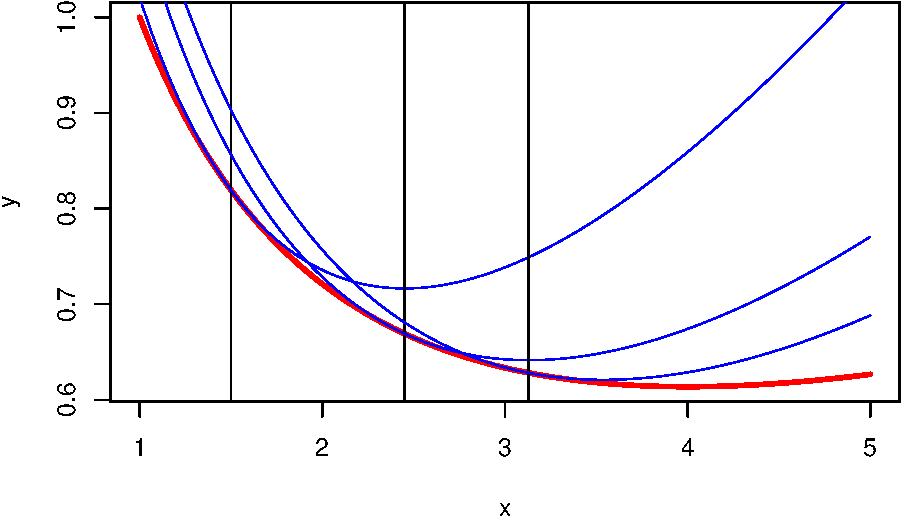
\includegraphics[keepaspectratio]{smacofIntro_files/figure-pdf/majplot-1.pdf}}
\end{center}

\sectionbreak

\section*{References}\label{references}
\addcontentsline{toc}{section}{References}

\phantomsection\label{refs}
\begin{CSLReferences}{1}{0}
\bibitem[\citeproctext]{ref-boehning_lindsay_88}
Böhning, D., and B. G. Lindsay. 1988. {``{Monotonicity of
Quadratic-approximation Algorithms}.''} \emph{Annals of the Institute of
Statistical Mathematics} 40 (4): 641--63.

\bibitem[\citeproctext]{ref-borg_groenen_05}
Borg, I., and P. J. F. Groenen. 2005. \emph{Modern Multidimensional
Scaling}. Second Edition. Springer.

\bibitem[\citeproctext]{ref-carroll_chang_70}
Carroll, J. D., and J. J. Chang. 1970. {``{Analysis of Individual
Differences in Multidimensional scaling via an N-way generalization of
"Eckart-Young" Decomposition.}''} \emph{Psychometrika} 35: 283--319.

\bibitem[\citeproctext]{ref-coombs_64}
Coombs, C. H. 1964. \emph{{A Theory of Data}}. Wiley.

\bibitem[\citeproctext]{ref-datorro_18}
Datorro, J. 2018. \emph{Convex Optimization and Euclidean Distance
Geometry}. Second Edition. Palo Alto, CA: Meebo Publishing.
\url{https://ccrma.stanford.edu/~dattorro/0976401304.pdf}.

\bibitem[\citeproctext]{ref-deleeuw_R_68g}
De Leeuw, J. 1968. {``Nonmetric Multidimensional Scaling.''} Research
Note 010-68. Department of Data Theory FSW/RUL.
\url{https://jansweb.netlify.app/publication/deleeuw-r-68-g/deleeuw-r-68-g.pdf}.

\bibitem[\citeproctext]{ref-deleeuw_B_73}
---------. 1973. {``Canonical Analysis of Categorical Data.''} PhD
thesis, University of Leiden, The Netherlands.
\url{https://jansweb.netlify.app/publication/deleeuw-b-73/deleeuw-b-73.pdf}.

\bibitem[\citeproctext]{ref-deleeuw_C_77}
---------. 1977. {``Applications of Convex Analysis to Multidimensional
Scaling.''} In \emph{Recent Developments in Statistics}, edited by J. R.
Barra, F. Brodeau, G. Romier, and B. Van Cutsem, 133--45. Amsterdam, The
Netherlands: North Holland Publishing Company.

\bibitem[\citeproctext]{ref-deleeuw_B_84}
---------. 1984. \emph{Canonical Analysis of Categorical Data}. Leiden,
The Netherlands: DSWO Press.
\url{https://jansweb.netlify.app/publication/deleeuw-b-84/deleeuw-b-84.pdf}.

\bibitem[\citeproctext]{ref-deleeuw_A_88b}
---------. 1988. {``Convergence of the Majorization Method for
Multidimensional Scaling.''} \emph{Journal of Classification} 5:
163--80.

\bibitem[\citeproctext]{ref-deleeuw_C_94c}
---------. 1994. {``{Block Relaxation Algorithms in Statistics}.''} In
\emph{Information Systems and Data Analysis}, edited by H. H. Bock, W.
Lenski, and M. M. Richter, 308--24. Berlin: Springer Verlag.
\url{https://jansweb.netlify.app/publication/deleeuw-c-94-c/deleeuw-c-94-c.pdf}.

\bibitem[\citeproctext]{ref-deleeuw_E_17e}
---------. 2017a. {``{Shepard Non-metric Multidimensional Scaling}.''}
2017.
\url{https://jansweb.netlify.app/publication/deleeuw-e-17-e/deleeuw-e-17-e.pdf}.

\bibitem[\citeproctext]{ref-deleeuw_E_17p}
---------. 2017b. {``{Tweaking the SMACOF Engine}.''} 2017.
\url{https://jansweb.netlify.app/publication/deleeuw-e-17-p/deleeuw-e-17-p.pdf}.

\bibitem[\citeproctext]{ref-deleeuw_heiser_C_77}
De Leeuw, J., and W. J. Heiser. 1977. {``Convergence of Correction
Matrix Algorithms for Multidimensional Scaling.''} In \emph{Geometric
Representations of Relational Data}, edited by J. C. Lingoes, 735--53.
Ann Arbor, Michigan: Mathesis Press.

\bibitem[\citeproctext]{ref-deleeuw_heiser_C_80}
---------. 1980. {``Multidimensional Scaling with Restrictions on the
Configuration.''} In \emph{Multivariate Analysis, Volume {V}}, edited by
P. R. Krishnaiah, 501--22. Amsterdam, The Netherlands: North Holland
Publishing Company.

\bibitem[\citeproctext]{ref-deleeuw_heiser_C_82}
---------. 1982. {``Theory of Multidimensional Scaling.''} In
\emph{Handbook of Statistics, Volume {II}}, edited by P. R. Krishnaiah
and L. Kanal. Amsterdam, The Netherlands: North Holland Publishing
Company.

\bibitem[\citeproctext]{ref-deleeuw_mair_A_09c}
De Leeuw, J., and P. Mair. 2009. {``{Multidimensional Scaling Using
Majorization: SMACOF in R}.''} \emph{Journal of Statistical Software} 31
(3): 1--30. \url{https://www.jstatsoft.org/article/view/v031i03}.

\bibitem[\citeproctext]{ref-dempster_laird_rubin_77}
Dempster, A. P., N. M. Laird, and D. B. Rubin. 1977. {``{Maximum
Likelihood for Incomplete Data via the EM Algorithm}.''} \emph{Journal
of the Royal Statistical Society} B39: 1--38.

\bibitem[\citeproctext]{ref-gifi_B_90}
Gifi, A. 1990. \emph{Nonlinear Multivariate Analysis}. New York, N.Y.:
Wiley.

\bibitem[\citeproctext]{ref-groenen_mathar_heiser_95}
Groenen, P. J. F., R. Mathar, and W. J. Heiser. 1995. {``{The
Majorization Approach to Multidimensional Scaling for Minkowski
Distances}.''} \emph{Journal of Classification} 12: 3--19.

\bibitem[\citeproctext]{ref-groenen_vandevelden_16}
Groenen, P. J. F., and M. Van de Velden. 2016. {``{Multidimensional
Scaling by Majorization: A Review}.''} \emph{Journal of Statistical
Software} 73 (8): 1--26.
\url{https://www.jstatsoft.org/index.php/jss/article/view/v073i08}.

\bibitem[\citeproctext]{ref-guttman_68}
Guttman, L. 1968. {``{A General Nonmetric Technique for Fitting the
Smallest Coordinate Space for a Configuration of Points}.''}
\emph{Psychometrika} 33: 469--506.

\bibitem[\citeproctext]{ref-harshman_70}
Harshman, R. A. 1970. {``{Foundations of the PARAFAC Procedure}.''}
Working Papers in Phonetics 16. UCLA.

\bibitem[\citeproctext]{ref-heiser_deleeuw_R_77}
Heiser, W. J., and J. De Leeuw. 1977. {``How to Use {SMACOF-I}.''}
Department of Data Theory FSW/RUL.

\bibitem[\citeproctext]{ref-kruskal_64a}
Kruskal, J. B. 1964a. {``{Multidimensional Scaling by Optimizing
Goodness of Fit to a Nonmetric Hypothesis}.''} \emph{Psychometrika} 29:
1--27.

\bibitem[\citeproctext]{ref-kruskal_64b}
---------. 1964b. {``{Nonmetric Multidimensional Scaling: a Numerical
Method}.''} \emph{Psychometrika} 29: 115--29.

\bibitem[\citeproctext]{ref-lange_16}
Lange, K. 2016. \emph{MM Optimization Algorithms}. SIAM.

\bibitem[\citeproctext]{ref-lethi_tao_18}
Le Thi, H. A., and P. D. Tao. 2018. {``{DC Programming and DCA: Thirty
Years of Developments}.''} \emph{Mathematical Programming, Series B}.

\bibitem[\citeproctext]{ref-lingoes_roskam_73}
Lingoes, J. C., and E. E. Roskam. 1973. {``{A Mathematical and Empirical
Analysis of Two Multidimensional Scaling Algorithms}.''}
\emph{Psychometrika} 38: Monograph Supplement.

\bibitem[\citeproctext]{ref-mair_groenen_deleeuw_A_22}
Mair, P., P. J. F. Groenen, and J. De Leeuw. 2022. {``{More on
Multidimensional Scaling in R: smacof Version 2}.''} \emph{Journal of
Statistical Software} 102 (10): 1--47.
\url{https://www.jstatsoft.org/article/view/v102i10}.

\bibitem[\citeproctext]{ref-mathar_meyer_94}
Mathar, R., and R. Meyer. 1994. {``Algorithms in Convex Analysis to Fit
l\_p -Distance Matrices.''} \emph{Journal of Multivariate Analysis} 51:
102--20.

\bibitem[\citeproctext]{ref-meulman_heiser_12}
Meulman, J. J., and W. J. Heiser. 2012. \emph{IBM SPSS Categories 21}.
IBM Corporation.

\bibitem[\citeproctext]{ref-nikolova_ng_05}
Niikolova, M., and M. Ng. 2005. {``Analysis of Half-Quadratic
Minimization Methods for Signal and Image Recovery.''} \emph{SIAM
Journal Scientific Computing} 27 (3): 937--66.

\bibitem[\citeproctext]{ref-ramsay_77}
Ramsay, J. O. 1977. {``{Maximum Likelihood Estimation in
Multidimensional Scaling}.''} \emph{Psychometrika} 42: 241--66.

\bibitem[\citeproctext]{ref-roskam_68}
Roskam, E. E. 1968. {``{Metric Analysis of Ordinal Data in
Psychology}.''} PhD thesis, University of Leiden.

\bibitem[\citeproctext]{ref-schoenberg_35}
Schoenberg, I. J. 1935. {``{Remarks to Maurice Frechet's article: Sur la
Definition Axiomatique d'une Classe d'Espaces Vectoriels Distancies
Applicables Vectoriellement sur l'Espace de Hllbert}.''} \emph{Annals of
Mathematics} 36: 724--32.

\bibitem[\citeproctext]{ref-shepard_62a}
Shepard, R. N. 1962a. {``{The Analysis of Proximities: Multidimensional
Scaling with an Unknown Distance Function. I}.''} \emph{Psychometrika}
27: 125--40.

\bibitem[\citeproctext]{ref-shepard_62b}
---------. 1962b. {``{The Analysis of Proximities: Multidimensional
Scaling with an Unknown Distance Function. II}.''} \emph{Psychometrika}
27: 219--46.

\bibitem[\citeproctext]{ref-takane_young_deleeuw_A_77}
Takane, Y., F. W. Young, and J. De Leeuw. 1977. {``Nonmetric Individual
Differences in Multidimensional Scaling: An Alternating Least Squares
Method with Optimal Scaling Features.''} \emph{Psychometrika} 42: 7--67.

\bibitem[\citeproctext]{ref-torgerson_58}
Torgerson, W. S. 1958. \emph{{Theory and Methods of Scaling}}. New York:
Wiley.

\bibitem[\citeproctext]{ref-torgerson_52}
Torgerson, W. S. 1952. {``{Multidimensional Scaling: I. Theory and
Method}.''} \emph{Psychometrika} 17 (4): 401--19.

\bibitem[\citeproctext]{ref-torgerson_65}
---------. 1965. {``{Multidimensional Scaling of Similarity}.''}
\emph{Psychometrika} 30 (4): 379--93.

\bibitem[\citeproctext]{ref-vandegeer_67}
Van de Geer, J. P. 1967. \emph{{Inleiding in de Multivariate Analyse}}.
Van Loghum Slaterus.

\bibitem[\citeproctext]{ref-vandegeer_71}
---------. 1971. \emph{{Introduction to Multivariate Analysis for the
Social Sciences}}. San Francisco, CA: Freeman.

\bibitem[\citeproctext]{ref-vosz_eckhardt_80}
Vosz, H., and U. Eckhardt. 1980. {``{Linear Convergence of Generalized
{W}eiszfeld's Method}.''} \emph{Computing} 25: 243--51.

\bibitem[\citeproctext]{ref-young_householder_38}
Young, G., and A. S. Householder. 1938. {``{Discussion of a Set of
Points in Terms of Their Mutual Distances}.''} \emph{Psychometrika} 3
(19-22).

\bibitem[\citeproctext]{ref-yuille_rangarajan_03}
Yuille, A. L., and A. Rangarajan. 2003. {``{The Concave-Convex
Procedure}.''} \emph{Neural Computation} 15: 915--36.

\bibitem[\citeproctext]{ref-zangwill_69a}
Zangwill, W. I. 1969. \emph{{Nonlinear Programming: a Unified
Approach}}. Englewood-Cliffs, N.J.: Prentice-Hall.

\end{CSLReferences}




\end{document}
